%!TeX root=Dissertation.tex
%%TC:ingore
\section{Background}
The aim of this project is to produce a small desktop application capable of analysing large sets of website log data for website owners in a convenient way. Every time a website receives a visitor various properties of their visit are recorded in the log files, for example their IP, the access time, the type of HTTP request sent by the visitor, and the user agent. These files can therefore become quite large and difficult to read. This is a lot of potentially useful data that website owners could miss out on; it is important to analyse these files so that any attacks can be identified and dealt with. It is now even easier for anyone to own their own website (see figure \ref{Number of Websites}), but there are very few solutions available for analysing web traffic.

\begin{figure}[H] \label{Number of Websites} 
    \centering
    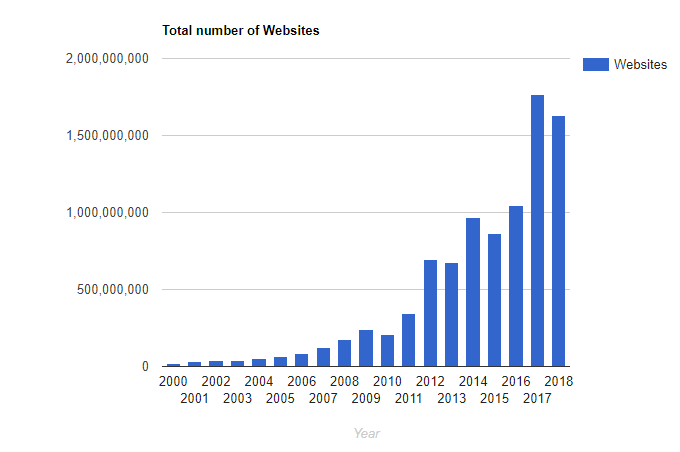
\includegraphics[width=\textwidth]{Images/numberOfWebsites.png}
    \caption{Total number of websites since 2000 (\cite{NumberofWebsites})}
    \label{Total number of websites since 2000}
\end{figure}
The majority of small businesses with a website are run by single individuals or small teams that do not necessarily have the time or resources to keep on top of their web traffic and potential attacks. The proposed application needs to account for the fact that these people will likely not have enough time to go through log files given their size. They also may not have the budget to buy solutions. It should be noted that a lot of web hosts do have automatic attack detection systems in place, as these are normally included in the cost of web hosting packages. However, many web hosts run a large number of servers, each of which often has a large volume of accounts. This can be seen in a recent article about cPanel's licensing update: Ryan Gray notes that 100 accounts in the early 2000s was a high number for one server, however now it is normal (\cite{cPanelArticle}). Due to their being more than one account on a server data would be aggregated to provide a overview of the server, therefore making some attacks harder to identify.

There are lots of different types of attack that can occur on a website. Some are easier to detect than others, for example, low bandwidth attacks are harder to detect. This was noted in 2014 by the National Research Council of Italy who say that "The problem is particularly challenging in virtue of the reduced amount of bandwidth generated by the attacks" (\cite{aiello2014line}). Therefore this implies that high bandwidth attacks are relatively easy to detect, so the focus of this dissertation will be to detect low bandwidth attacks and some other common attacks on websites that shall be discussed later. The findings will then be presented not to the server owner, but to the website owner so that they can be more informed about what is happening on their website.

The idea for this project came from when my own business website was attacked. I was fully prepared for a DDOS attack, however I found that there was an IP coming onto my site around 20 times in a minute that would then go away for a number of hours only to return some time later. The only way that I was able to detect this attack was by reading through that month's log file, which contained a few thousand lines of website logs, and comparing this to spikes in the server load. I felt that it would be helpful if there was a program to analyse the data. The only solutions out there were for large corporations, there wasn't anything for individual sites. There are also websites that monitor for suspicious IP addresses, for example https://www.abuseipdb.com/, however, as these would not take a server log file, you would need to input IP addresses one by one. Also, due to the fact the information is readily available online, the attackers know when they have been identified as a suspicious IP address and can easily change their IP address. Therefore there is a need for a solution that relies upon that background data but doesn't reveal what is known about an IP address. 

There is a vast amount of data in log files, although there are many limitations of the data held in these log files. They will record IP addresses however they can not record the location of those IP addresses. While there are tools such as google analytics that provide very detailed data on visitors to the site, these tools automatically filter out bots and do not show activity if the user generates an error. Another limitation of the log file comes from looking at the user agent field, whilst this records whether it is a bot, for example, google bot, this can be easily faked, and the log file cannot detect a fake google bot. Therefore, a fake google bot is a common form of attack (\cite{algiryage2018distinguishing}), due to the fact that the server cannot verify that it is a google bot.

The program will need to be easy to use for a non-expert website owner. Most website owners are computer literate however may not know how to access or analyse this type of data. Many website owners use content management systems (CMS). WordPress already has a lot of plugins available for security, and while these do a good job at blocking attacks in real-time and preventing invalid logins, they are not able to look at data over longer periods. The program aims to be compatible with all websites but due to the popularity of CMSs and wide variety of attack types, even websites that don't run a CMS  because of their market dominance (at time of writing, about 60\% of websites use WordPress (\cite{IsItWP})), may encounter these attacks without being aware.
\section{Proposed Work}
\label{proposed}
The work proposed is to write a piece of software, that will aid website management and detect attacks. The software must be easy to use, therefore the proposed work will also look at issues around user experience and interface design. The finished software should have some kind of self learning mechanism therefore should include a database to store some data. 

The software will be written in Java, this is due to the fact that it is architecturally neutral, meaning that the software can be run on any machine. Java also makes it easy to design simple graphical user interfaces so that the user can interact with the software. Other languages were considered such as C, due to the fact that it runs on many Unix systems, which most webservers run. This was discounted due to the fact that most website owners will not have access to the servers themselves. In addition to this, C will not be as easy to implement a user interface on, as I have no experience in writing graphical user interfaces in C. 

The database will be run on Microsoft Access, this is due to the fact Java has an extensive library for interacting with Microsoft Access. I already have experience writing Java applications with Microsoft Access, therefore this will speed up development times. I will be able to quickly integrate the program with Microsoft Access. 

One concern that will need to be addressed in this dissertation centres around the usability of the program. Are users actually able to analyse and take action on the data? Or is it inherently too complicated for a program to be worth writing? Even within the program there will be limitations on how the data will be analysed and presented to the user, and the program would be designed not to take decisions for the user but to present the data in a more understandable manner. Therefore, would the user take the necessary action, and would they even know what action to take? Work done by Ben-Asher and Gonzalez looks at whether cyber security knowledge is needed to detect attacks (\cite{ben2015effects}). This concern will be addressed by looking at relevant literature and may also include some user testing of the software. The user testing component will focus primarily on the usability of the software rather than looking at the outputs that the user gets.

The literature review will also include a critical analysis on current technologies to detect attacks. This literature will help guide the development of the software by illuminating the gaps that exist in current technology. I will also look at whether network architecture can help to stop potential attacks. For example, services such as CloudFlare use an 'Anycast' network, wherein every server on the network has the same IP address, so that when a DDOS attack occurs they can spread the attack over many servers. The attacker cannot tell that they are not all going to the same server (\cite{CloudFlare}). CloudFlare could offer solutions to detect low bandwidth attacks as well. This will be investigated in more detail in the literature review. One potential solution could be for CloudFlare to ask, 'is this user requesting a big enough chunk of data from the website to be defined as legitimate?'. My literature review will answer whether this will work in practice.

I intend to develop the software using agile techniques. In other words, rather than fully writing the software first and then testing it, the software will be tested as throughout the development process. This will help to make the development time shorter as errors in the code will be fixed before the next stage of the software is written. 

\section{Aims and Objectives}
For this project I will have several aims and objectives.
\subsection{Aims}
\begin{enumerate}
    \item Develop a system that is able to identify different types of website attacks and provide the user with an easy to understand report on this.
    \item To be able to crowd-source data so that the system is able to keep its knowledge about different IPs and the risk that they may be carrying out an attack up-to-date.
    \item To keep the data about IPs out of the view of the general public so that the attackers are less able to know if they have been found to be suspicious.
\end{enumerate}

\subsection{Objectives}
\begin{enumerate}
    \item Carry out a literature review and produce requirements documentation
    \begin{enumerate}
        \item Review of common attack techniques and how difficult or easy they are to detect.
        \item Review literature on how to present information to users on website data.
    \end{enumerate}
    \item Review of current protection that is available and how much data these programs release to the end user.
    \begin{enumerate}
        \item Look for attack prevention solutions for CMSs.
        \item Look for the reliability and ease of use for current attack prevention solutions.
    \end{enumerate}
    \item Produce relevant system documentation.
    \begin{enumerate}
        \item Produce relevant class diagram.
        \item Produce relevant Entity Relationship Diagrams (using crow's feet notation). 
        \item Produce relevant state transition diagram for interesting behaviour.
    \end{enumerate}
    \item Evaluate the project after completion.
    \begin{enumerate}
        \item Carry out a detailed test plan on the product.
        \item Check for usability with non-technical users.
    \end{enumerate}
    \item Abstract and introduction.
\end{enumerate}

\section{Skills}
For this project I will need several skills that I either already have and will develop or new skills that I will need to learn. Where I do not have the skill required I will consult learning tutorials and online literature in order to increase my knowledge. 

This project will require both networking and program skills. The networking skills will be important to ensure that I understand what the IP information tells us. This will need to be fed into the Java program in a way that is easy for the user to understand, and is not too big O complex due to the potential size of the data that could be submitted. 
\begin{enumerate}
\item Java 
\begin{enumerate}
    \item Java will form the main component of the project. I will therefore need to understand Java to a high enough standard to implement the program. Due to the complexities of the program using the right data structures to enable a quick response will be key to the program. 
    \item The majority of my modules have involved the use of Java. Even the modules that did not contain Java as a programming language helped me to develop a conceptual understanding of programming due to the concepts being similar across the board.
\end{enumerate}
\item Microsoft access SQL
\begin{enumerate}
    \item The main data for the project will be stored in a database, therefore it will be necessary to ensure that my SQL skills are up to scratch in order to store the data correctly and then the retrieval of the correct information will be crucial for this project. Some of the SQL queries may be complex in nature, for example nested queries may be needed.
    \item The module that most helped with SQL was the 'Relational Database' module, which covered the foundation of SQL databases, however SQL databases have also been used in the web modules and with Java in the 'Software Engineering Practice' module. \end{enumerate}
\item Networking Knowledge
\begin{enumerate}
    \item I have a basic understanding of networking and how networks work. I will need to learn how to apply this knowledge to detect attacks.
    \item I have gained some networking knowledge in the 'Computer Networks' module. 
    \item The majority of my working knowledge of networks, particularly the internet, came from my placement year, as I had to work with a variety of different websites and provide solutions to stop attacks. Nonetheless, my networking knowledge in identifying attacks is still limited and will need to be improved. 
\end{enumerate}
\item Time Management Skills
\begin{enumerate}
    \item As this is the largest project that I will work on during my undergraduate degree, I will need to manage my time well to ensure that I can get the work done and keep up with the other modules that I am taking this year. 
    \item I learnt a lot of time management skills in the 'Software Engineering' practical module. I will further develop these by asking my supervisor for advice early on and by researching time management techniques that work well for dissertation-style projects.
\end{enumerate}
\end{enumerate}

\section{Resources}

\subsection{Hardware}
\begin{enumerate}
    \item A PC - to write the software on.
\end{enumerate}
\subsection{Software}
\begin{enumerate}
    \item LAMP stack - a LAMP stack is needed to run websites on.
    \item Log files in the extended format
\end{enumerate}

\section{Structure and Contents of the Report}
\subsection{Report Structure}
\begin{enumerate} [topsep=0pt,itemsep=-0ex,partopsep=1ex,parsep=1pt,leftmargin=7ex,label=CH.\arabic*]
     \item Introduction
     \item Review of current detection methods
     \item Tools and packages 
     \item Requirements Specifications
     \item Testing
     \item conclusions
\end{enumerate}

\subsection{List of Appendices}
\begin{enumerate} [label=\Alph*)]
    \item Terms of Reference
    \item Ethics form
    \item Risk Assessment
    \item Use case diagrams and  descriptions
    \item ERD
    \item Data dictionary
    \item Class Diagram 
\end{enumerate}
\section{Marking Scheme: Software Engineering Project }
\textbf{Overview}

\begin{enumerate} [topsep=0pt,itemsep=-0ex,partopsep=1ex,parsep=1pt,label=]
    \item Report: 40\%
\begin{enumerate}[topsep=0pt,itemsep=-1ex,partopsep=1ex,parsep=1ex,label=]
\item Abstract \& Introduction 	5\%
\item Analysis 			30\%
\item Synthesis 			30\%
\item  Evaluation \& Conclusions 	30\%
\item Presentation 			5\%
\end{enumerate}
\item Product 50\%
\begin{enumerate}[topsep=0pt,itemsep=-1ex,partopsep=1ex,parsep=1ex,label=]
\item Fitness for Purpose 		40\%
\item Build Quality 			60\%
\end{enumerate}
\item Viva 10\%
\end{enumerate}

\clearpage

\section{Project Plan}
\noindent
\rotatebox{90}{%!TeX root=TermsOfReference.tex

% A lot of the settings here are tuned to fit a landscape gantt chart into
% an A4 piece of paper.
\begin{ganttchart}[
time slot format=little-endian,
calendar week text=\currentweek,
x unit=2.4pt,
y unit chart=14pt,
y unit title=12pt,
title label font=\scriptsize,
bar top shift=.15,
bar height=0.7,
milestone label font = \small,
group label font = {\tiny\bfseries},
group inline label node/.append style=centered,
hgrid=true,vgrid={*6{draw=none},dotted},
region/.style={inline,group peaks width=2,
  group peaks height=0.25, group height=0.5,
  group top shift=0.2 ,group/.append style={fill=#1}},
milestone left shift=0,
milestone right shift=1,
ms/.style={inline,
    milestone inline label node/.append style={#1=0pt}}
]{11/9/19}{18/05/20} %<- Dates Gantt Chart runs from and to

\gantttitlecalendar{year,month,week=1}\\
% Highlight Smesters and Vactions
\ganttgroup[region=blue!10]{Sem 1}{23/9/19}{20/12/19}
\ganttgroup[region=red!50]{Christmas}{20/12/17}{1/1/18}
\ganttgroup[region=blue!50]{Sem 2}{15/1/20}{23/3/20}
\ganttgroup[region=green!25]{Easter}{26/3/20}{13/4/20}
\ganttgroup[region=blue!50]{Sem 2}{16/04/20}{27/04/20}\\

% Project Deadlines (from the slides)
\ganttmilestone[]{TOR}{28/10/19}
\ganttmilestone[ms=left]{\bfseries TOR}{28/10/19}
\ganttmilestone[ms=right]{Draft Analysis}{6/12/19}
\ganttmilestone[ms=left]{Submit}{30/4/20}
\ganttnewline[thick]

% --Tasks go here
% put in a title, a start date, end date...
\ganttbar{TOR}{23/9/19}{21/10/19}
\ganttbar[inline]{\emph{revise}}{25/10/19}{10/11/19}\\
\ganttbar{Analysis}{18/9/19}{24/11/19}\\
\ganttbar{Design}{31/10/19}{17/1/20}\\
\ganttbar{Build}{17/1/20}{17/2/20}\\
\ganttbar{Test}{20/2/20}{16/3/20}\\
\ganttmilestone[ms=right]{Build complete}{18/2/20}
\end{ganttchart}
}
%%TC:endingore